%%%%%%%%%%%%%%%%%%%%%%%%%%%%%%%%%%%%%%%%%
% Beamer Presentation
% LaTeX Template
% Version 1.0 (10/11/12)
%
% This template has been downloaded from:
% http://www.LaTeXTemplates.com
%
% License:
% CC BY-NC-SA 3.0 (http://creativecommons.org/licenses/by-nc-sa/3.0/)
%
%%%%%%%%%%%%%%%%%%%%%%%%%%%%%%%%%%%%%%%%%

%----------------------------------------------------------------------------------------
%	PACKAGES AND THEMES
%----------------------------------------------------------------------------------------

\documentclass{beamer}

\mode<presentation> {

% The Beamer class comes with a number of default slide themes
% which change the colors and layouts of slides. Below this is a list
% of all the themes, uncomment each in turn to see what they look like.

%\usetheme{default} % +
%\usetheme{AnnArbor}
%\usetheme{Antibes}
%\usetheme{Bergen}
%\usetheme{Berkeley} % +
%\usetheme{Berlin}
%\usetheme{Boadilla} % +
%\usetheme{CambridgeUS}
%\usetheme{Copenhagen}
%\usetheme{Darmstadt}
%\usetheme{Dresden} 
%\usetheme{Frankfurt} % +
%\usetheme{Goettingen}
%\usetheme{Hannover}
%\usetheme{Ilmenau}
%\usetheme{JuanLesPins}
%\usetheme{Luebeck}
%\usetheme{Madrid} % +
%\usetheme{Malmoe}
%\usetheme{Marburg}
%\usetheme{Montpellier}
%\usetheme{PaloAlto}
%\usetheme{Pittsburgh}
%\usetheme{Rochester}
\usetheme{Singapore} % +
%\usetheme{Szeged}
%\usetheme{Warsaw}

% As well as themes, the Beamer class has a number of color themes
% for any slide theme. Uncomment each of these in turn to see how it
% changes the colors of your current slide theme.

%\usecolortheme{albatross}
%\usecolortheme{beaver}
%\usecolortheme{beetle}
%\usecolortheme{crane}
%\usecolortheme{dolphin}
%\usecolortheme{dove}
%\usecolortheme{fly}
%\usecolortheme{lily}
%\usecolortheme{orchid}
%\usecolortheme{rose}
%\usecolortheme{seagull}
%\usecolortheme{seahorse}
%\usecolortheme{whale}
%\usecolortheme{wolverine}

%\setbeamertemplate{footline} % To remove the footer line in all slides uncomment this line
%\setbeamertemplate{footline}[page number] % To replace the footer line in all slides with a simple slide count uncomment this line

%\setbeamertemplate{navigation symbols}{} % To remove the navigation symbols from the bottom of all slides uncomment this line
}

\usepackage{graphicx} % Allows including images
\usepackage{booktabs} % Allows the use of \toprule, \midrule and \bottomrule in tables
\usepackage{caption}
\usepackage{subcaption}

%----------------------------------------------------------------------------------------
%	TITLE PAGE
%----------------------------------------------------------------------------------------

\title[Epidemics Wokrshop]{G-CSC Epidemics group\newline An introduction to disease modelling via SEIRD}

\author{\textcolor{blue}{Yannick Rosam, Tristan Scheidemann, Marvin Glaser\\}
\vspace{2mm}\footnotesize{Special Thanks: Devansh Rastogi}} % Your name
\institute[G-CSC] % Your institution as it will appear on the bottom of every slide, may be shorthand to save space
{
Goethe Universtiy Frankfurt - Center for Scientific Computing \\ % Your institution for the title page
\medskip
%\textit{john@smith.com} % Your email address
}
%\date{\today} % Date, can be changed to a custom date

\begin{document}

%----------------------------------------------------------------------------------------
%	PRESENTATION SLIDES
%----------------------------------------------------------------------------------------

\begin{frame}
\titlepage % Print the title page as the first slide
\end{frame}

%----------------------------------------------------------------------------------------

\begin{frame}
\frametitle{Overview} 
\tableofcontents 
\end{frame}

%----------------------------------------------------------------------------------------
%	SECTION FORMATING
%----------------------------------------------------------------------------------------

%\AtBeginSection[]{
%  \begin{frame}
%  \vfill
%  \centering
%  \begin{beamercolorbox}[sep=8pt,center,shadow=true,rounded=true]{title}
%    \usebeamerfont{title}\insertsectionhead\par%
%  \end{beamercolorbox}
%  \vfill
%  \end{frame}
%}

%----------------------------------------------------------------------------------------

\section{Theory I}

\subsection{Situation}
\begin{frame}
	\frametitle{Situation}
	\begin{enumerate}
		\item diseases are not nice\\\vspace{0.1cm}
	         			

		\item  infectious diseases are doubly not nice \\\vspace{0.1cm}
	       	
                \item infectious diseases in todays interconnected world are horrible	\\\vspace{0.1cm}
         		
	\end{enumerate}
\end{frame}

\begin{frame}
	\frametitle{Situation}
	\begin{enumerate}
		\item diseases are not nice\\\vspace{0.1cm}
	         			
		\item  infectious diseases are doubly not nice \\\vspace{0.1cm}
	       	
                \item infectious diseases in todays interconnected world are horrible	\\\vspace{0.1cm}
	\end{enumerate}

\textbf{Question:} Are we able to broadly understand their behavior?

\end{frame}

\begin{frame}
	\frametitle{Situation}
	\begin{itemize}
		\item Infectious disease models can give quantitative answers\\\vspace{0.1cm}
	         			
		\item  Although not perfect, results can guide policy \\\vspace{0.1cm}
	       	
                \item Won't yield insights into disease itself but its effect on society	\\\vspace{0.1cm}
	\end{itemize}

\end{frame}

\subsection{Simulator}
\begin{frame}
	\frametitle{}
	\begin{itemize}
		\item The \textbf{EpidemicsRunner} developed by the G-CSC allows the user to test various scenarios and relate these models to the real world
	         			
		\item  The user can define scenarios... \\\vspace{0.1cm}
	       	
                \item ...and fit the models to real life data	\\\vspace{0.1cm}

	\end{itemize}

\end{frame}


\begin{frame}
The EpidemicsRunner is quick response guidance tool, that allows a non-expert user to quickly
simulate various epidemics scenarios based on real data.

\end{frame}

\begin{frame}
	\frametitle{SEIRD Model}
	\begin{itemize}
		\item The (S)usceptible (E)xposed (I)nfected (R)ecovered (D)eaths model is a well known framework to model the spread of infectious diseases		
		\item  It is the simplest model found in EpidemicsRunner \\\vspace{0.1cm}
	       	
                \item Is a robust basis for other more specialized models	\\\vspace{0.3cm}

	\end{itemize}
	%\begin{center}
	%	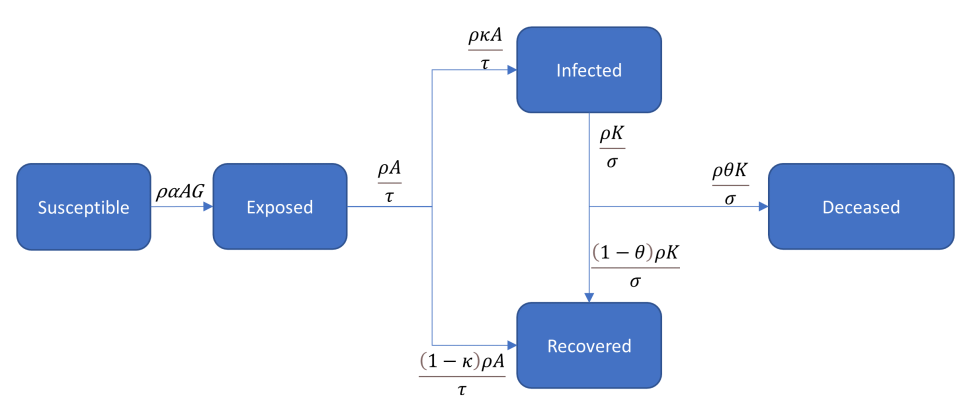
\includegraphics[width=0.7\textwidth]{./images/SEIRD_flow.png}
	%\end{center}
\end{frame}

\begin{frame}
	\frametitle{SEIRD Classes}
	\begin{description}
		\item[Susceptibles]
	        These are people that have never had the disease
 			
		\item[Exposed]
	       	These are people that have been exposed to the disease, are able to transmit it
                but have no yet been quarantined (i.e. show no symptoms yet)

                \item[Infected]
                These are people that have previously been exposed and are now sick with the disease.
                They are also quarantined and cannot infect any other person

               \item[Recovered]
                These are people that have previously been exposed or infected and are now  considered disease-free (recovered). 

               \item[Deaths]
                These are people that have previously been infected and are now dead

	\end{description}

\end{frame}

\begin{frame}
	\frametitle{SEIRD Model (ODE)}
\begin{equation} \label{eq1}
\begin{split}
\frac{dS}{dt} & = -\alpha SE \\
\frac{dE}{dt} & = \alpha SE-\frac{1}{qq}E\\
\frac{dI}{dt} & = \frac{\kappa}{qq} E-\frac{1}{qq}I\\
\frac{dR}{dt} & = \frac{(1-\kappa)}{qq} E+\frac{(1-\theta)}{pp}I\\
\frac{dD}{dt} & = \frac{\theta}{pp} I\\
\end{split}
\end{equation}	

\end{frame}

%----------------------------------------------------------------------------------------

\section{Practial I}

\begin{frame}
\frametitle{ODE Widget - Overview}
	\begin{centering}
		\vspace{0.79cm}
		\includegraphics<1>[scale=0.275]{./images/ODE_a0.png}
		\includegraphics<2>[scale=0.275]{./images/ODE_a1.png}
		\includegraphics<3>[scale=0.275]{./images/ODE_a2.png}
		\includegraphics<4>[scale=0.275]{./images/ODE_a3.png}
		\includegraphics<5>[scale=0.275]{./images/ODE_a4.png}
	\end{centering}
\end{frame}

\begin{frame}
\frametitle{Live "modelling" session 1} 
	Lets model $\alpha$ for  two different scenarios:\\\vspace{0.3cm}
	\begin{enumerate}
		\item Bellcurve:\\\vspace{0.1cm}
			\begin{tabular}{| c | c |}
				\hline
				Infected & 82000 \\
				\hline
				Exposed & 8147 \\
				\hline
				timeframe & 81 days \\
				\hline
			\end{tabular} \vspace{0.5cm}

		\item Rapid growth:\\\vspace{0.1cm}
			\begin{tabular}{| c | c |}
				\hline
				Infected & 82000 \\
				\hline
				Exposed & 1755 \\
				\hline
				timeframe & 64 days \\
				\hline
			\end{tabular}
	\end{enumerate}
\end{frame}
%----------------------------------------------------------------------------------------

\section{Theory II}

\subsection{Solvers}
\begin{frame}
\frametitle{Solvers} 
	stuff about sovers
\end{frame}

\subsection{Partial differential equations}
\begin{frame}
	\frametitle{Partial differential Equations (PDE)} 
	basic info about PDE model
\end{frame}

%----------------------------------------------------------------------------------------

\section{Practical II}
\begin{frame}
	\frametitle{The PDE widget - Overview} 
	\begin{centering}
		\vspace{0.2cm}
		\includegraphics<1>[scale=0.275]{./images/PDE0.png}
		%\vspace{-0.1cm}
		\includegraphics<2>[scale=0.275]{./images/PDE1.png}
		%\vspace{-0.05cm}
		\includegraphics<3>[scale=0.275]{./images/PDE2.png}
		\vspace{-0.19cm}
		\includegraphics<4>[scale=0.275]{./images/PDE3.png}
		\includegraphics<5>[scale=0.275]{./images/PDE4.png}
	\end{centering}
\end{frame}

\begin{frame}
\frametitle{Live "modelling" seesion 2} 
	show of very small stepsize for effect?\\
	with/without diffusion?\\
	show of movie of small stepsize
\end{frame}

%----------------------------------------------------------------------------------------
\section{Application}
\subsection{Previous Work}
\begin{frame}
\frametitle{Modelling Covid in Germany} 
	\begin{columns}
		\begin{column}{0.45\textwidth}
			\vspace{-4cm}
			\begin{enumerate}[$\bullet$]
				\item<2-> We started out with a grid of Germany.
			\vspace{0.5cm}
				\item<3> But of course, once you have a gird...
			\end{enumerate}
		\end{column}
		\begin{column}{0.45\textwidth}
			\centering
			\includegraphics<2->[width=\textwidth]{./images/ger.png}
		\end{column}
	\end{columns}
\end{frame}

\begin{frame}
\frametitle{Modelling Covid in Germany} 
	\centering{
		\vspace{-0.5cm}
		\onslide<1->{...you can play with the model}
		\vspace{0.5cm}
	}
	\begin{columns}
		\begin{column}{0.45\textwidth}
			\centering
			\onslide<2->{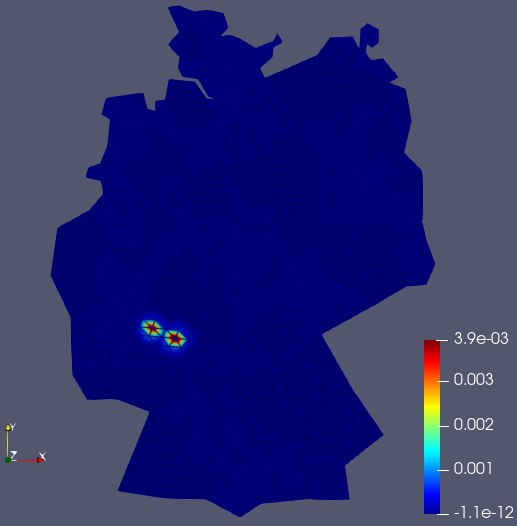
\includegraphics[width=\textwidth]{./images/d_grid_fw.png}
			reasonable parameters}
		\end{column}
		\begin{column}{0.45\textwidth}
			\centering
			\onslide<3>{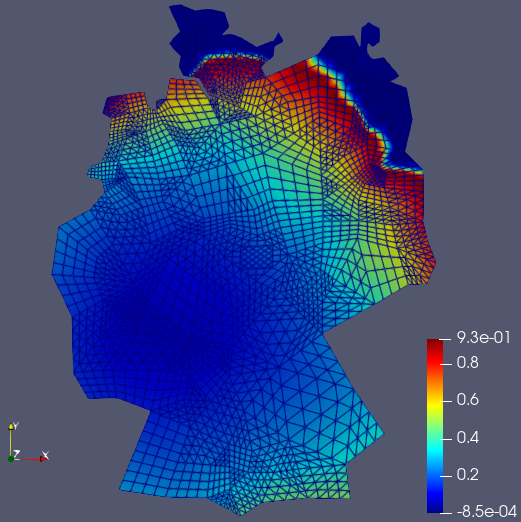
\includegraphics[width=\textwidth]{./images/d_grid_wave.png}
			not so reasonable parameters}
		\end{column}
	\end{columns}
\end{frame}

\begin{frame}
\frametitle{Modelling Covid in Germany} 
	\begin{columns}
		\begin{column}{0.45\textwidth}
			\begin{enumerate}[$\bullet$]
				\onslide<1->{\item Of course we also did some serious modelling}
				\onslide<2>{\item PDE model for seven cities in Germany
					\begin{enumerate}[-]
						\item Hannover
						\item Heinsberg
						\item Frankfurt
						\item Wiesbaden
						\item Stuttgart
						\item M\"unchen
						\item Berlin
					\end{enumerate}
					}
			\end{enumerate}
		\end{column}
		\begin{column}{0.40\textwidth}
			\centering
			\includegraphics<1>[width=\textwidth]{./images/d_grid.png}
			\includegraphics<2>[width=\textwidth]{./images/d_grid2.png}
		\end{column}
	\end{columns}
\end{frame}

\begin{frame}
\frametitle{Modelling Covid in Germany} 
	\begin{columns}
		\hspace{-0.5cm}
		\begin{column}{0.5\textwidth}
			\centering
			\onslide<1->{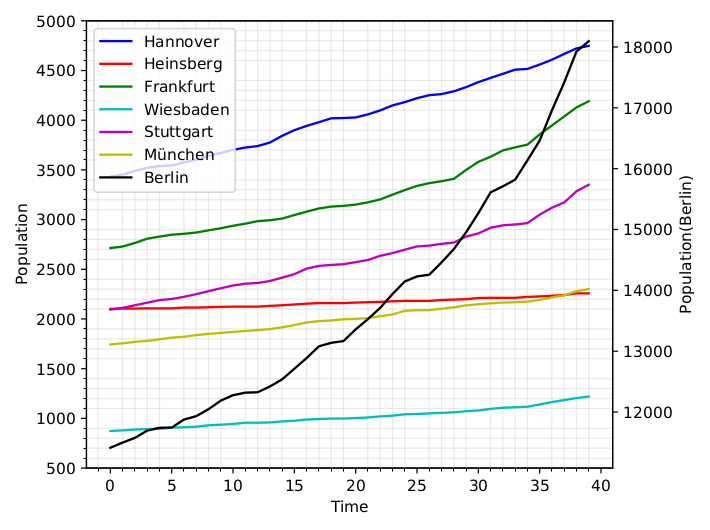
\includegraphics[width=\textwidth]{./images/city_orig.png}
			Real world infection cases}
		\end{column}
		%\hspace{1cm}
		\begin{column}{0.5\textwidth}
			\centering
			\onslide<2>{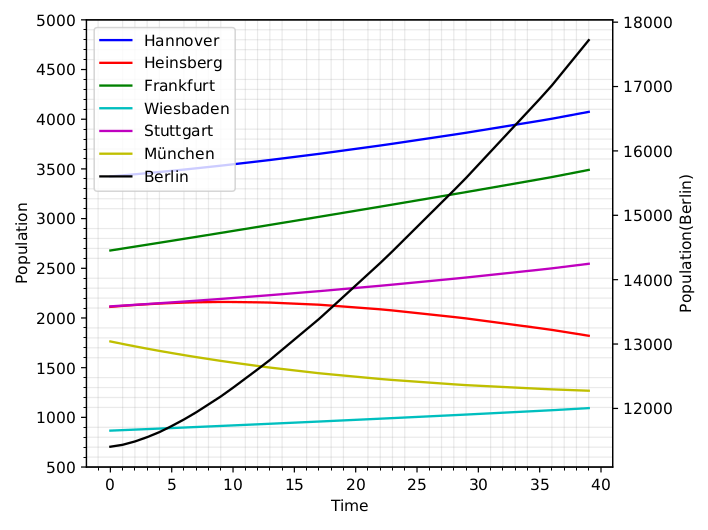
\includegraphics[width=\textwidth]{./images/city_model.png}
			Modelled infection cases}
		\end{column}
	\end{columns}
\end{frame}
%----------------------------------------------------------------------------------------

\subsection{Outlook}

\begin{frame}
\frametitle{Big and small ideas for applications} 
	\vspace{-1cm}
	\onslide<2->{
		Future topics:
		\begin{enumerate}[$\bullet$]
			\item Modelling of smaller areas with finer grid [in progress]
			\item Use the model in differenct scenarios (countries, diseases, ...)
			\item Compare SEIRD with statistical models
		\end{enumerate}
	}
			
	\vspace{0.3cm}
	\onslide<3->{
		Current applications:
		\begin{enumerate}[$\bullet$]
			\item Public health management (easy modelling of scenarios)
			\item Use SEIRD to  prepare for future Epidemics/Pandemics (Supplies, Beds, Employees)
			\item Study and understand the mechanics of disease spreading
		\end{enumerate}
	}
\end{frame}
%----------------------------------------------------------------------------------------

\begin{frame}
\frametitle{Questions, Answers and Discussions} 
	\centering{
	\textbf{Thank you for your attention and for hosting this event!}
}
\end{frame}
%------------------------------------------------


\end{document} 
